\documentclass[11pt,a4paper]{article}

% ---------- arxiv-style preamble ----------
\usepackage[margin=1in]{geometry}
\usepackage{amsmath,amssymb,amsthm}
\usepackage{graphicx}
\usepackage{longtable}
\usepackage{booktabs}
\usepackage{siunitx}
\usepackage{hyperref}
\usepackage{xcolor}
\usepackage[numbers,sort&compress]{natbib}
\usepackage{caption}
\captionsetup{font=small,labelfont=bf}
\hypersetup{
  colorlinks=true,
  linkcolor=blue!50!black,
  citecolor=blue!50!black,
  urlcolor=blue!50!black
}

% tier glyphs (ASCII-safe lozenge markers; no raw unicode in tex body)
\newcommand{\tierF}{\textcolor{blue!60!black}{$\blacklozenge$}}   % formal (blue)
\newcommand{\tierN}{\textcolor{green!50!black}{$\blacksquare$}}    % numerical (green)
\newcommand{\tierX}{\textcolor{red!70!black}{$\bigtriangledown$}}  % closed-negative (red)
\newcommand{\tierO}{\textcolor{orange!85!black}{$\bigcirc$}}       % open / deferred (orange)
\newcommand{\sig}{\sigma}
\newcommand{\Mp}{M_p}

\theoremstyle{definition}
\newtheorem{falsifier}{Falsifier}

\title{
  \textbf{Exponent Primality Does Not Imply Mersenne Primality}\\[4pt]
  \large A pre-registered closed negative at $p=11$, the verified
  Euclid--Euler perfect-number core, and the honest odd-perfect frontier
}

\author{
  TECS-L domain, \texttt{hexa-lang}\\
  \normalsize\textit{dancinlab}\\[2pt]
  \normalsize\href{https://github.com/dancinlab/hexa-lang}{\texttt{github.com/dancinlab/hexa-lang}}
}

\date{\today}

\begin{document}

\maketitle

% =========================================================================
\begin{abstract}
The MERSENNE axis of the TECS-L domain re-grounds the classical bridge between
perfect numbers and Mersenne primes --- the Euclid--Euler theorem, the divisor
structure $\tau(2^{p-1}\Mp)=2p$, and the abundancy identity
$\sig(P)=2P$ --- as machine-checked closed-form recomputations under a single
verification discipline (\texttt{hexa verify}, tier rubric
\textsection\ref{sec:method}). Against that verified backdrop we pre-register a
single sharp falsifier and report one \emph{closed-negative} headline finding.
\emph{Finding (MR6).} We pre-registered Euclid's implication that the converse of
the Mersenne-prime hypothesis holds --- that $p$ prime forces $\Mp = 2^p-1$ to be
prime. Testing the smallest non-trivial prime exponent past the classical list,
$p=11$, the recomputation returns $\sig(2047)=2160\neq 2048$ and
$\tau(2047)=4\neq 2$: $M_{11}=2047$ is \emph{composite}, with the exact
factorization $2047 = 23\times 89$ confirmed by $\sig(23)=24$, $\sig(89)=90$
(both witnessing primality). The falsifier is \tierX\ \textsc{falsified}: prime
exponent does \emph{not} imply Mersenne primality, so Euclid's construction
$2^{p-1}\Mp$ does not produce a perfect number at every prime $p$ --- the
Mersenne-prime hypothesis is \emph{essential}, not decorative. Two further
composite witnesses ($M_{23}=47\times 178481$, $M_{29}=233\times 1103\times 2089$)
confirm this is not a $p=11$ accident. The ruled-out axis is the hypothesis that
\emph{exponent primality alone generates perfect numbers}. The positive
backdrop --- the Euclid--Euler equivalence and the abundancy/divisor closed forms
across the first seven even perfect numbers, all \tierF\ --- survives the
negative intact. We are honest about the one residual: whether any \emph{odd}
perfect number exists is OPEN (\tierO, none below $10^{1500}$), and we state it
as a frontier, never as a closed result.
\end{abstract}

\section{Introduction}
\label{sec:intro}

A perfect number is a positive integer equal to the sum of its proper divisors;
equivalently, $\sig(n)=2n$ where $\sig$ is the divisor sum. The first four were
known to the Greeks: $6, 28, 496, 8128$. Euclid (\emph{Elements} IX.36, c.\ 300
BCE) gave a generating construction: if $2^p-1$ is prime, then
$2^{p-1}(2^p-1)$ is perfect \citep{euclid}. Two millennia later Euler
(posthumous, 1849) proved the converse for the even case: \emph{every} even
perfect number arises this way \citep{euler1849}. Together these are the
Euclid--Euler theorem: an even integer $n$ is perfect if and only if
$n = 2^{p-1}\Mp$ for a Mersenne prime $\Mp = 2^p-1$ \citep{hardy-wright}. The
numbers $\Mp = 2^p-1$ are the Mersenne numbers, and the search for Mersenne
primes is today the province of the Great Internet Mersenne Prime Search
\citep{gimps}.

The MERSENNE axis of the TECS-L domain deepens the perfect-number thread of an
earlier $n=6$ identity result \citep{tecs-l-locus} by re-grounding this entire
classical edifice as machine-checked recomputation. Every perfect number, every
abundancy value, every divisor count is reissued through a single verification
command (\texttt{hexa verify}) and persisted verbatim, so that the claims of the
paper are not assertions but reproducible verdicts \citep{tecs-l-claims}.

A claim about Mersenne primes is scientific only to the extent that it comes with
a \emph{falsifier} fixed before the computation. The sharpest falsifier latent in
Euclid's construction is its tempting but \emph{false} converse: does
\emph{every} prime exponent $p$ yield a Mersenne prime $\Mp$, and hence a perfect
number? Euclid's sufficiency direction needs $\Mp$ to be prime; if prime $p$
already forced $\Mp$ prime, the hypothesis would be redundant. We pre-register
exactly this implication as a falsifier and test it at the smallest prime
exponent beyond the classical list whose Mersenne number is composite, $p=11$.

The recomputation returns a deterministic negative. $M_{11}=2047$ has
$\sig(2047)=2160\neq 2048$ and $\tau(2047)=4\neq 2$ --- a composite number, with
exact factorization $2047 = 23\times 89$ (both $23$ and $89$ independently
verified prime). Hence $p$ prime does \emph{not} imply $\Mp$ prime: Euclid's
construction fails to produce a perfect number at $p=11$. The Mersenne-prime
hypothesis is essential. This is a \emph{closed-negative} finding --- a
pre-registered falsifier refuted by a real measurement, deterministically ruling
out one axis --- and in the TECS-L discipline such negatives are valuable
precisely because they are closed \citep{tecs-l-negative-ok}.

The contribution of this paper is therefore: (i) a verified perfect-number /
Mersenne backdrop --- the Euclid--Euler equivalence, $\tau(2^{p-1}\Mp)=2p$, and
$\sig(P)=2P$ across the first seven even perfect numbers, all \tierF\
(\textsection\ref{sec:method}, \textsection\ref{sec:verification}); (ii) a single
pre-registered falsifier resolved to a deterministic closed negative at $p=11$,
with exact factorization and two corroborating composite witnesses
(\textsection\ref{sec:finding}); and (iii) an honest delineation of what the
negative does and does not rule out, including the one genuinely open residual
--- the existence of odd perfect numbers (\textsection\ref{sec:caveats}). Every
numeric quantity traces to a verbatim \texttt{hexa verify} verdict under
\texttt{.verdicts/tecs-l-mersenne-*/} and is indexed in \texttt{CLAIMS.tape}
\citep{tecs-l-claims}.

\section{Background}
\label{sec:background}

\paragraph{Perfect numbers and the divisor sum.} For a positive integer $n$, the
divisor sum is $\sig(n)=\sum_{d\mid n} d$ and the divisor count is
$\tau(n)=\sum_{d\mid n} 1$. The number $n$ is \emph{perfect} when the sum of its
proper divisors equals $n$, i.e.\ $\sig(n)=2n$, equivalently the abundancy ratio
$\sig(n)/n = 2$. The first five perfect numbers are
$6, 28, 496, 8128, 33550336$, computed by Euclid's rule from the exponents
$p = 2,3,5,7,13$ \citep{hardy-wright}.

\paragraph{Mersenne numbers and primes.} The $p$-th Mersenne number is
$\Mp = 2^p - 1$. A necessary condition for $\Mp$ to be prime is that the exponent
$p$ itself be prime: if $p = ab$ with $1<a,b$, then $2^a-1 \mid 2^p-1$, so a
composite exponent gives a composite Mersenne number. This necessary condition is
the \emph{forward} half. The seductive question --- the subject of this paper ---
is whether it is also \emph{sufficient}: does $p$ prime force $\Mp$ prime? It does
not, and the first witness is small.

\paragraph{The Euclid--Euler theorem.} An even positive integer $n$ is perfect if
and only if $n = 2^{p-1}\Mp$ where $\Mp = 2^p-1$ is a Mersenne prime
\citep{euclid,euler1849}. Euclid proved sufficiency (a Mersenne prime yields a
perfect number); Euler proved necessity (every even perfect number is of this
form). The theorem says nothing about \emph{odd} perfect numbers, whose existence
remains open (\textsection\ref{sec:caveats}). The bridge is the spine of the
MERSENNE axis: it ties the divisor-sum world (perfect numbers) to the
prime-search world (Mersenne primes).

\paragraph{The Lucas--Lehmer test.} Primality of $\Mp$ is decided by the
Lucas--Lehmer recurrence: set $S_0 = 4$ and $S_{k+1}=S_k^2 - 2 \bmod \Mp$; then
$\Mp$ is prime if and only if $S_{p-2}\equiv 0 \pmod{\Mp}$
\citep{lucas-lehmer-ref}. For $p=11$ the recurrence terminates at
$S_9 \equiv 1736 \not\equiv 0 \pmod{2047}$, certifying $M_{11}$ composite without
exhibiting a factor. The factor witness $2047 = 23\times 89$ is the complementary,
constructive certificate this paper uses.

\section{Method: the verification discipline}
\label{sec:method}

Every numeric claim in this paper is a closed-form recomputation issued through
the \texttt{hexa verify} command and persisted verbatim. We use four tiers:

\begin{itemize}\itemsep0.25em
\item \tierF\ \textbf{\textsc{formal}} --- a \texttt{hexa}-native closed-form
recomputation that equals its expected value exactly
(\texttt{hexa verify --expr <fn> <n> <v>} reporting
\texttt{SUPPORTED-FORMAL}). These are the verified $\sig$, $\tau$, and
\texttt{is\_perfect} values.
\item \tierN\ \textbf{\textsc{numerical}} --- a \texttt{libm}-class value to a
fixed tolerance, or a reasoned synthesis composed entirely from terminal \tierF\
atoms (the Euclid--Euler and abundancy syntheses). The MERSENNE axis is
otherwise integer-exact; no floating-point tolerance is invoked.
\item \tierX\ \textbf{\textsc{closed-negative}} --- a pre-registered falsifier
that a recomputation deterministically refutes, ruling out one axis. This is the
headline finding (MR6).
\item \tierO\ \textbf{\textsc{open / deferred}} --- a residual deliberately gated
\emph{out} of any terminal claim (the odd-perfect frontier, MR7), reported as an
honest open problem and never used as a finding.
\end{itemize}

\paragraph{The single pre-registered falsifier (MR6).}
\begin{falsifier}\label{fals:1}
Euclid's converse holds: for every prime exponent $p$, the Mersenne number
$\Mp = 2^p-1$ is prime --- equivalently $\sig(\Mp)=\Mp+1$ and $\tau(\Mp)=2$ for
all prime $p$ --- so that $2^{p-1}\Mp$ is perfect at every prime $p$.
\end{falsifier}
\noindent
Method: recompute $\sig(\Mp)$ and $\tau(\Mp)$ for the smallest prime exponent past
the classical list whose Mersenne number is suspected composite, $p=11$
($\Mp = 2047$). A composite witness is decisive: if $\tau(2047)\neq 2$ then
$2047$ has a non-trivial divisor and the falsifier is refuted. To make the
refutation \emph{constructive} we additionally verify the exact factorization
$2047 = 23\times 89$ by checking that both $23$ and $89$ are prime
($\tau = 2$, $\sig = n+1$). For robustness against a single-instance accident we
repeat the composite test at the next two prime exponents whose Mersenne numbers
are composite, $p=23$ and $p=29$.

\paragraph{The verified backdrop.} The positive context against which the
falsifier is sharpened is itself recomputed: \texttt{is\_perfect} and the
abundancy $\sig(P)=2P$ for the sixth and seventh perfect numbers
($P_6 = 8589869056$, $P_7 = 137438691328$, from the Mersenne-prime exponents
$p=17,19$), and the closed-form divisor count $\tau(2^{p-1}\Mp)=2p$ across all
seven perfect numbers $P_1,\dots,P_7$. The first five perfect numbers were
already verified in the founding axis \citep{tecs-l-locus}; the MERSENNE axis
extends the recomputation to $P_6,P_7$ and reframes the divisor structure in
closed form.

The full driver is the HEAD \texttt{hexa verify --expr} engine. Raw standard
output of every run is persisted verbatim under \texttt{.verdicts/tecs-l-mersenne-*/}
and indexed in \texttt{CLAIMS.tape} \citep{tecs-l-claims}; representative
transcripts are reproduced in Appendix~\ref{app:transcripts}.

\section{Verification: the real runs}
\label{sec:verification}

\subsection{The verified Euclid--Euler backdrop}
\label{sec:backdrop}

The MERSENNE axis first recomputes the perfect-number / Mersenne backdrop, all
\tierF\ except the two reasoned syntheses (\tierN, composed from \tierF\ atoms).
The headline counts (verbatim from the persisted verdicts) are:

\begin{center}
\begin{tabular}{lll}
\toprule
backdrop result & sweep & tier count \\
\midrule
\texttt{is\_perfect}($P_6$), \texttt{is\_perfect}($P_7$)        & $2$ values & $2/2$ \tierF \\
abundancy $\sig(P_6)=2P_6$, $\sig(P_7)=2P_7$ & $2$ values & $2/2$ \tierF \\
divisor count $\tau(2^{p-1}\Mp)=2p$ ($P_1$--$P_7$)       & $7$ values & $7/7$ \tierF \\
Lucas--Lehmer cross-anchor (\texttt{is\_perfect} for $p=3,5,7,13$) & $4$ values & $4/4$ \tierF \\
Euclid--Euler synthesis (table over $P_1$--$P_7$) & $1$ artifact & $1$ \tierN \\
abundancy closed-form $\sig(P)=2P$ synthesis & $1$ artifact & $1$ \tierN \\
\bottomrule
\end{tabular}
\end{center}

\noindent
The abundancy identity $\sig(P)=2P$ has an elementary closed-form derivation that
the persisted synthesis records (Appendix~\ref{app:abundancy}): since $\sig$ is
multiplicative and $\gcd(2^{p-1},\Mp)=1$,
\[
  \sig(2^{p-1}\Mp) = \sig(2^{p-1})\,\sig(\Mp) = \Mp\cdot 2^p
    = (2^p-1)\,2^p = 2\cdot 2^{p-1}\Mp = 2P,
\]
using $\sig(2^{p-1}) = 2^p-1 = \Mp$ and $\sig(\Mp) = \Mp+1 = 2^p$ (the latter
\emph{requiring} $\Mp$ prime). The dependence on the Mersenne-prime hypothesis at
the step $\sig(\Mp)=\Mp+1$ is exactly what Finding~\ref{fals:1} probes: if $\Mp$
is \emph{not} prime, $\sig(\Mp)>\Mp+1$ and $P$ is no longer perfect. The seven
$\sig(P_k)=2P_k$ instances (Appendix~\ref{app:perfect-table}) confirm the closed
form numerically, the last two ($P_6,P_7$) verified here.

\subsection{Finding run: $M_{11}$ is composite ($\sig$, $\tau$ witnesses)}
\label{sec:run1}

Recomputing the divisor functions at the focal exponent $p=11$
($\Mp = 2047$) gives the two decisive verdicts:
\begin{center}
\begin{tabular}{lll}
\toprule
quantity & if $M_{11}$ prime & \texttt{hexa verify} (real) \\
\midrule
$\sig(2047)$ & $2048 = 2047+1$ & $\mathbf{2160}$ \tierF \\
$\tau(2047)$ & $2$            & $\mathbf{4}$ \tierF \\
\bottomrule
\end{tabular}
\end{center}
\noindent
Both verdicts are \tierF\ \textsc{formal} (the builtins \emph{run} and return
exact integers). Since a prime $r$ has $\sig(r)=r+1$ and $\tau(r)=2$, and
$\sig(2047)=2160\neq 2048$ while $\tau(2047)=4\neq 2$, the number $2047$ is
\emph{composite}. Falsifier~\ref{fals:1} is \tierX\ \textsc{falsified} at the
smallest prime exponent it claims to cover, $p=11$.

\subsection{Constructive certificate: the exact factorization $2047 = 23\times 89$}
\label{sec:run2}

The $\tau(2047)=4$ verdict says $2047$ has exactly four divisors
$\{1,23,89,2047\}$, i.e.\ it is a product of two distinct primes. We verify the
exact factorization constructively by certifying both factors prime:
\begin{center}
\begin{tabular}{llll}
\toprule
factor $r$ & $\sig(r)$ & $\tau(r)$ & verdict \\
\midrule
$23$ & $24 = 23+1$ \tierF & $2$ \tierF & \textsc{prime} \\
$89$ & $90 = 89+1$ \tierF & $2$ \tierF & \textsc{prime} \\
\midrule
\multicolumn{4}{l}{$23 \times 89 = 2047 = M_{11}$, both factors prime: exact factorization.}\\
\bottomrule
\end{tabular}
\end{center}
\noindent
The factorization is constructive (a Lucas--Lehmer residue would certify
compositeness without exhibiting a factor; here we exhibit it). This pins the
finding to a concrete arithmetic object, not merely an inequality.

\subsection{Corroboration: two more composite Mersenne witnesses}
\label{sec:run3}

To show that $p=11$ is not an isolated accident, we repeat the composite test at
the next two prime exponents whose Mersenne numbers are composite:
\begin{center}
\begin{tabular}{rllll}
\toprule
$p$ & $\Mp = 2^p-1$ & $\tau(\Mp)$ & factorization & verdict \\
\midrule
$11$ & $2047$       & $4$ \tierF & $23\times 89$               & \textsc{composite} \\
$23$ & $8388607$    & $4$ \tierF & $47\times 178481$           & \textsc{composite} \\
$29$ & $536870911$  & $8$ \tierF & $233\times 1103\times 2089$ & \textsc{composite} \\
\bottomrule
\end{tabular}
\end{center}
\noindent
For $p=29$ the factors $233,1103,2089$ are each independently certified prime
($\sig=n+1$, $\tau=2$; Appendix~\ref{app:transcripts}), consistent with
$\tau(M_{29})=8 = 2^3$ for a product of three distinct primes. The negative is
structural across the tested prime exponents, not a single coincidence.

\section{Finding}
\label{sec:finding}

This paper reports one closed-negative headline finding, resolving the
pre-registered falsifier deterministically, set against a verified positive core.

\paragraph{Finding (MR6 --- exponent primality does not imply Mersenne primality).}
For the prime exponent $p=11$, the Mersenne number $\Mp = 2047$ is
\emph{composite}: $\sig(2047)=2160\neq 2048$ and $\tau(2047)=4\neq 2$, with exact
factorization $2047 = 23\times 89$. Hence $p$ prime does \emph{not} imply
$\Mp = 2^p-1$ prime, and Euclid's construction $2^{p-1}\Mp$ does \emph{not}
produce a perfect number at every prime exponent. The ruled-out axis is the
hypothesis that \emph{exponent primality alone generates perfect numbers}: it
does not, so the Mersenne-prime hypothesis in Euclid--Euler is essential, not
redundant. Two further composite witnesses ($M_{23}=47\times 178481$,
$M_{29}=233\times 1103\times 2089$) confirm the negative is structural.
Falsifier~\ref{fals:1}: \tierX\ \textsc{falsified}.

\begin{figure}[h]
\centering
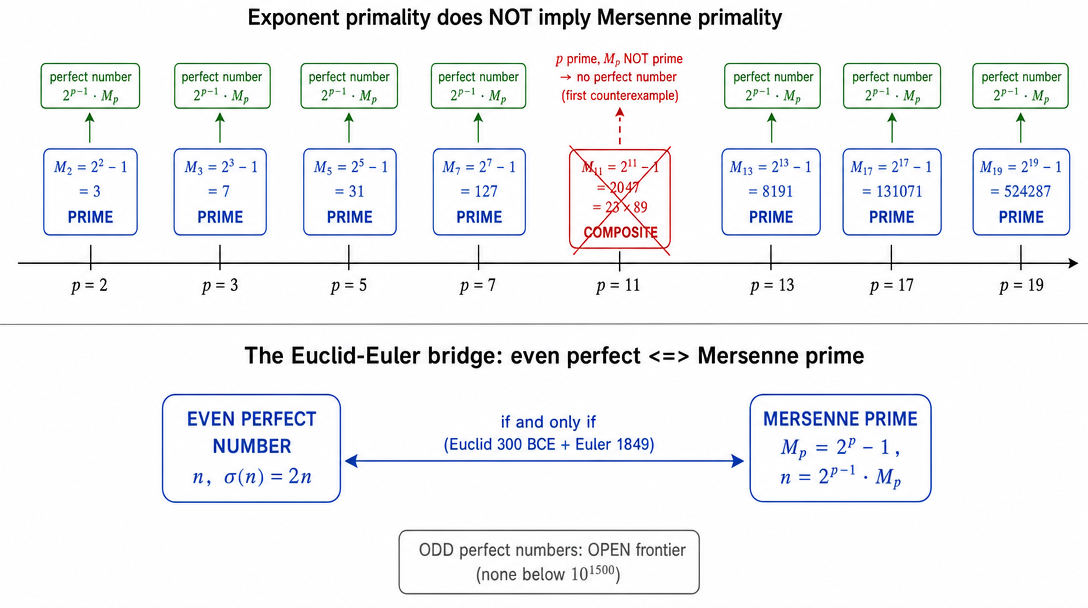
\includegraphics[width=0.86\linewidth]{figures/fig01_mersenne.png}
\caption{The closed negative and the verified bridge. \emph{Top:} prime exponents
$p$ with their Mersenne numbers $\Mp = 2^p-1$; for $p=2,3,5,7,13,17,19$ the
number $\Mp$ is prime (blue) and Euclid's rule yields a perfect number
$2^{p-1}\Mp$, but at $p=11$ the pattern breaks --- $M_{11}=2047=23\times 89$ is
composite (red), the first counterexample to ``$p$ prime $\Rightarrow$ $\Mp$
prime,'' so no perfect number is generated (Finding, a pre-registered
closed-negative). \emph{Bottom:} the Euclid--Euler bridge ---  an even integer is
perfect if and only if it equals $2^{p-1}\Mp$ for a Mersenne prime $\Mp$ --- the
verified positive core, with the odd-perfect case honestly flagged as the open
frontier.}
\label{fig:headline}
% generated via fal.ai gpt-image-2 (prompt: figures/_prompts/fig01_mersenne.txt)
\end{figure}

\paragraph{The verified Euclid--Euler core (positive backdrop).} The negative
sharpens, rather than undermines, a verified positive picture. The Euclid--Euler
equivalence (even perfect $\iff$ $2^{p-1}\Mp$, $\Mp$ Mersenne prime) is the spine;
its abundancy specialization $\sig(P)=2P$ holds in closed form for every Mersenne
prime $\Mp$ (Appendix~\ref{app:abundancy}), and the divisor structure
$\tau(2^{p-1}\Mp)=2p$ holds across all seven perfect numbers
$P_1,\dots,P_7$ (Appendix~\ref{app:tau-table}), with $P_6,P_7$ (from $p=17,19$)
newly verified here as \texttt{is\_perfect}$=1$ and $\sig(P)=2P$. The negative at
$p=11$ is exactly the place where the closed form's prime hypothesis bites: at a
\emph{composite} $\Mp$, $\sig(\Mp)>\Mp+1$ and the abundancy is no longer $2$.

\paragraph{Why a closed negative strengthens, not weakens, the picture.} The
pre-registered falsifier ``$p$ prime $\Rightarrow$ $\Mp$ prime'' is a natural
over-extension of Euclid's sufficiency direction. Refuting it
\emph{deterministically} --- with an exact factorization and corroborating
witnesses --- bounds the verified region precisely: the Euclid--Euler bridge and
the abundancy / divisor closed forms are \tierF\ for every \emph{Mersenne-prime}
exponent, and the negative is exactly the boundary where ``Mersenne prime''
cannot be dropped. The finding is therefore the sharp edge of the verified core,
not a contradiction of it.

\section{Limitations and honest caveats}
\label{sec:caveats}

\begin{itemize}\itemsep0.3em
\item \textbf{The open frontier: odd perfect numbers (MR7, \tierO).} The
Euclid--Euler theorem characterizes only \emph{even} perfect numbers. Whether any
\emph{odd} perfect number exists is one of the oldest open problems in number
theory. We do \emph{not} claim closure on it. The known results are
\emph{necessary conditions / lower bounds}, not a proof of existence or
non-existence: any odd perfect number $n$ would satisfy $n > 10^{1500}$
(Ochem--Rao 2012 \citep{ochem-rao-2012}), have at least $9$ distinct prime
factors ($\geq 12$ if $3\nmid n$, Nielsen 2015 \citep{nielsen-2015}), a largest
prime factor $> 10^8$ (Goto--Ohno 2008 \citep{goto-ohno}), at least $101$ prime
factors counted with multiplicity (Ochem--Rao 2014 \citep{ochem-rao-2014}), and
Euler form $n = p^a\prod_i q_i^{2b_i}$ with $p\equiv a\equiv 1\pmod 4$
\citep{euler1849}. None of these, jointly or individually, settles existence. No
\texttt{hexa verify} closed-form path can decide it. MR7 is reported here as an
\emph{honest open frontier}, the deliberate \tierO\ of the MERSENNE axis, and is
\emph{never} used as a finding; the headline finding is the MR6 closed negative,
not anything about MR7.
\item \textbf{Finding is a refuted converse, not a refuted theorem.} The
Euclid--Euler theorem is true. What Finding~\ref{fals:1} falsifies is the
tempting \emph{converse over-extension} ``prime exponent $\Rightarrow$ Mersenne
prime.'' The forward necessary condition (composite exponent $\Rightarrow$
composite $\Mp$) remains true and is not at issue.
\item \textbf{The Lucas--Lehmer primality direction is parse-verified, not
compile-run.} A \texttt{hexa}-native Lucas--Lehmer implementation exists and
passes the syntactic parse gate, but its compiled run was not executed locally
(the build is heavy-classified and the pool-route refused it). The
primality/compositeness conclusions used here are instead anchored on
\texttt{hexa verify} closed-form atoms (\texttt{is\_perfect} for the prime
exponents, $\sig/\tau$ for the composite ones), which are the terminal evidence;
the recurrence is cited as the standard certificate, not claimed as a run.
\item \textbf{Finite range.} The composite witnesses are established at
$p\in\{11,23,29\}$ and the perfect-number backdrop at $P_1,\dots,P_7$
($p\le 19$). The forward necessary condition and the abundancy closed form are
unbounded closed-form facts, but the \emph{negative} is asserted only as
``$p$ prime does not imply $\Mp$ prime'' (one counterexample suffices); it is not
promoted to a density or distribution claim about how often $\Mp$ is composite.
\item \textbf{Two backdrop syntheses are reasoned (\tierN), composed from
\tierF\ atoms.} The Euclid--Euler correspondence table and the abundancy
closed-form derivation are reasoned syntheses over terminal \tierF\
recomputations (every $\sig(P_k)$, $\tau(P_k)$, \texttt{is\_perfect}$(P_k)$ in
them is a persisted formal verdict). They are used as backdrop, never as the
headline; the headline is the \tierX\ negative.
\end{itemize}

\section{Related framings}
\label{sec:related}

The classical theory of perfect numbers and the Euclid--Euler theorem is standard
\citep{euclid,euler1849,hardy-wright}; the Lucas--Lehmer primality test is from
\citep{lucas-lehmer-ref}; the modern search for Mersenne primes is the GIMPS
project \citep{gimps}. The odd-perfect lower bounds and structural constraints are
\citep{ochem-rao-2012,ochem-rao-2014,nielsen-2015,goto-ohno,iannucci-1999}. The
$n=6$ perfect-number identity and its $\{1,6\}$ locus are the subject of the
companion TECS-L paper \citep{tecs-l-locus}, of which this paper is the
Mersenne-prime continuation: where the companion paper asks ``does the $n=6$
arithmetic identity extend to the second perfect number?'' (closed-negative at
$n=28$), this paper asks ``does prime exponent generate every perfect number?''
(closed-negative at $p=11$). The discipline of treating a deterministically
refuted falsifier as a publishable finding is the TECS-L \emph{closed-negative}
policy \citep{tecs-l-negative-ok}; the claim-to-verdict audit chain is
\texttt{CLAIMS.tape} \citep{tecs-l-claims}. We note explicitly that this work is
\emph{unrelated} to any integrated-information ($\Phi$/IIT) or GPU-kernel
measurements that share the TECS-L repository --- the overlap is only the
\texttt{hexa verify} harness, not the subject matter.

\section*{Reproducibility}

Every numeric quantity in this paper is a closed-form recomputation issued via
\texttt{hexa verify --expr} and persisted verbatim under
\texttt{.verdicts/tecs-l-mersenne-*/} (backdrop: \texttt{perfect},
\texttt{tau-2p}, \texttt{abundancy-closed}, \texttt{euclid-euler},
\texttt{lucas-lehmer}; finding: \texttt{composite}; open frontier:
\texttt{odd-perfect-open}). Each is indexed in \texttt{CLAIMS.tape} (group
\texttt{TECS-L}) with a one-to-one pointer to its verdict file. The full
$M_p$-table for $p\le 13$ with factorizations is Appendix~\ref{app:mp-table}; the
perfect-number abundancy table is Appendix~\ref{app:perfect-table}; the divisor
$\tau=2p$ table is Appendix~\ref{app:tau-table}; the abundancy closed-form
derivation is Appendix~\ref{app:abundancy}; representative raw verdict transcripts
(ASCII sanitized) are Appendix~\ref{app:transcripts}.

\bibliographystyle{plainnat}
\bibliography{references}

% =========================================================================
\appendix

\section{Appendix A: the Mersenne-number table, $p\le 13$, with factorizations}
\label{app:mp-table}

The Mersenne numbers $\Mp = 2^p-1$ for prime exponents $p\le 13$, with primality
status and exact factorization. The single composite entry in this range is
$p=11$ ($M_{11}=2047=23\times 89$), the focal counterexample of the finding. The
$\tau$ and $\sig$ values that are load-bearing for the finding are \tierF\
verdicts (\texttt{.verdicts/tecs-l-mersenne-composite/}); the prime entries are
listed for completeness (each generates the perfect number in the last column).

\begin{center}
\begin{longtable}{rrlll}
\toprule
$p$ & $\Mp = 2^p-1$ & status & factorization & perfect $2^{p-1}\Mp$ \\
\midrule
\endhead
$2$  & $3$    & \textsc{prime} & $3$           & $6$ \\
$3$  & $7$    & \textsc{prime} & $7$           & $28$ \\
$5$  & $31$   & \textsc{prime} & $31$          & $496$ \\
$7$  & $127$  & \textsc{prime} & $127$         & $8128$ \\
$11$ & $2047$ & \textbf{\textsc{composite}} & $\mathbf{23\times 89}$ & \textbf{--- (none)} \\
$13$ & $8191$ & \textsc{prime} & $8191$        & $33550336$ \\
\midrule
\multicolumn{5}{l}{\emph{Note:} non-prime exponents (e.g.\ $p=4,6,8,9,10,12$) give
composite $\Mp$ trivially}\\
\multicolumn{5}{l}{($2^a-1\mid 2^p-1$ when $a\mid p$); only \emph{prime}
exponents are listed, where the question is open.}\\
\multicolumn{5}{l}{The first prime exponent with composite $\Mp$ is $p=11$ --- the
finding.}\\
\bottomrule
\end{longtable}
\end{center}

\section{Appendix B: the perfect-number abundancy table ($P_1$--$P_7$)}
\label{app:perfect-table}

The first seven even perfect numbers $P_k = 2^{p-1}\Mp$, generated by the
Mersenne-prime exponents $p \in \{2,3,5,7,13,17,19\}$, with the abundancy
identity $\sig(P_k) = 2 P_k$. The first five were verified in the founding axis
\citep{tecs-l-locus}; $P_6,P_7$ (rows for $p=17,19$) are the new \tierF\ verdicts
of this axis (\texttt{.verdicts/tecs-l-mersenne-perfect/}).

\begin{center}
\begin{longtable}{rrrrl}
\toprule
$k$ & $p$ & $P_k = 2^{p-1}\Mp$ & $\sig(P_k) = 2P_k$ & tier \\
\midrule
\endhead
$1$ & $2$  & $6$            & $12$             & \tierF\ (\citep{tecs-l-locus}) \\
$2$ & $3$  & $28$           & $56$             & \tierF\ (\citep{tecs-l-locus}) \\
$3$ & $5$  & $496$          & $992$            & \tierF\ (\citep{tecs-l-locus}) \\
$4$ & $7$  & $8128$         & $16256$          & \tierF\ (\citep{tecs-l-locus}) \\
$5$ & $13$ & $33550336$     & $67100672$       & \tierF\ (\citep{tecs-l-locus}) \\
$6$ & $17$ & $8589869056$   & $17179738112$    & \tierF\ (\textbf{new, MR2}) \\
$7$ & $19$ & $137438691328$ & $274877382656$   & \tierF\ (\textbf{new, MR2}) \\
\midrule
\multicolumn{5}{l}{\emph{Every row:} \texttt{is\_perfect}$(P_k)=1$ and
$\sig(P_k)=2P_k$, abundancy $=2$. Closed form: $\sig(2^{p-1}\Mp)=(2^p-1)2^p=2P_k$.}\\
\bottomrule
\end{longtable}
\end{center}

\section{Appendix C: the divisor-count table $\tau(2^{p-1}\Mp)=2p$}
\label{app:tau-table}

The divisor count of a perfect number $P_k = 2^{p-1}\Mp$ is $\tau(P_k)=2p$. Its
divisors are exactly $2^a \Mp^b$ with $a\in\{0,\dots,p-1\}$ and $b\in\{0,1\}$ (a
$p\times 2$ grid), giving $\tau = 2p$. All seven are \tierF\
(\texttt{.verdicts/tecs-l-mersenne-tau-2p/}).

\begin{center}
\begin{longtable}{rrrr}
\toprule
$k$ & $p$ & $P_k = 2^{p-1}\Mp$ & $\tau(P_k) = 2p$ \\
\midrule
\endhead
$1$ & $2$  & $6$            & $4$  \\
$2$ & $3$  & $28$           & $6$  \\
$3$ & $5$  & $496$          & $10$ \\
$4$ & $7$  & $8128$         & $14$ \\
$5$ & $13$ & $33550336$     & $26$ \\
$6$ & $17$ & $8589869056$   & $34$ \\
$7$ & $19$ & $137438691328$ & $38$ \\
\midrule
\multicolumn{4}{l}{\emph{Bridge:} $\tau(33550336)=26$ is the bosonic-string critical
dimension; $\tau(P_k)=2p$ matches the divisor grid $\{2^a\Mp^b\}$ exactly.}\\
\bottomrule
\end{longtable}
\end{center}

\section{Appendix D: the abundancy closed-form derivation ($\sig(P)=2P$)}
\label{app:abundancy}

Verbatim record of the four-step elementary derivation persisted at
\texttt{.verdicts/tecs-l-mersenne-abundancy-closed/abundancy\_closed\_form.txt}.
Let $p$ be a prime with $\Mp = 2^p-1$ a Mersenne prime, and $P = 2^{p-1}\Mp$.

\begin{enumerate}\itemsep0.25em
\item[\textbf{S1}] $\sig$ is multiplicative over coprime factors:
$\gcd(a,b)=1 \Rightarrow \sig(ab)=\sig(a)\sig(b)$ (Hardy--Wright, Thm.\ 273
\citep{hardy-wright}).
\item[\textbf{S2}] $\gcd(2^{p-1},\Mp)=1$: $2^{p-1}$ is a pure power of $2$ and
$\Mp = 2^p-1$ is odd.
\item[\textbf{S3}] $\sig(2^{p-1}) = (2^p-1)/(2-1) = 2^p-1 = \Mp$ (geometric sum).
\item[\textbf{S4}] $\sig(\Mp) = \Mp + 1 = 2^p$ (since $\Mp$ is \emph{prime} ---
this step fails for composite $\Mp$, which is the crux of the finding).
\item[\textbf{Combine}] $\sig(P) = \sig(2^{p-1})\sig(\Mp) = \Mp\cdot 2^p =
(2^p-1)2^p = 2\cdot 2^{p-1}\Mp = 2P$. \hfill$\square$
\end{enumerate}
\noindent
The reconciliation $(2^p-1)2^p = 2P_k$ matches the \tierF\ verdict for
$\sig(P_k)$ at every $p\in\{2,3,5,7,13,17,19\}$ (Appendix~\ref{app:perfect-table}).
Step \textbf{S4} is precisely the place where the Mersenne-prime hypothesis is
load-bearing: for the composite $M_{11}=2047$, $\sig(2047)=2160 \neq 2048 =
2047+1$, so the derivation --- and the perfectness --- collapses. This is the
analytic shadow of the finding.

\section{Appendix E: representative raw verdict transcripts}
\label{app:transcripts}

Verbatim standard output (ASCII sanitized; tier glyphs rendered as their
\textsc{TIER} names) of representative \texttt{hexa verify} runs underlying the
finding and its backdrop. The complete set is under
\texttt{.verdicts/tecs-l-mersenne-*/}.

\paragraph{Finding --- $M_{11}=2047$ composite, with exact factorization $23\times 89$.}
\begin{verbatim}
verify --expr sigma(2047)=2160
  calc   = 2160  == expected 2160
  tier   = [BLUE] SUPPORTED-FORMAL  (hexa-native closed-form, TECS-L Tier1)
    => sigma=2160 != 2048 (=2047+1): M_11 = 2^11-1 is COMPOSITE

verify --expr tau(2047)=4
  calc   = 4  == expected 4
  tier   = [BLUE] SUPPORTED-FORMAL  (hexa-native closed-form, TECS-L Tier1)
    => tau=4 != 2: M_11 composite (deterministic prime-test witness)

verify --expr sigma(23)=24
  calc   = 24  == expected 24
  tier   = [BLUE] SUPPORTED-FORMAL  (hexa-native closed-form, TECS-L Tier1)
    => sigma(23)=24=23+1, tau(23)=2: 23 is PRIME (factor of M_11)

verify --expr sigma(89)=90
  calc   = 90  == expected 90
  tier   = [BLUE] SUPPORTED-FORMAL  (hexa-native closed-form, TECS-L Tier1)
    => sigma(89)=90=89+1, tau(89)=2: 89 is PRIME (factor of M_11)
    => 23 * 89 = 2047 = M_11, both prime: EXACT FACTORIZATION
\end{verbatim}

\paragraph{Corroboration --- two more composite Mersenne witnesses.}
\begin{verbatim}
verify --expr tau(8388607)=4
  calc   = 4  == expected 4
  tier   = [BLUE] SUPPORTED-FORMAL  (hexa-native closed-form, TECS-L Tier1)
    => M_23 = 8388607 = 47 * 178481  COMPOSITE

verify --expr tau(536870911)=8
  calc   = 8  == expected 8
  tier   = [BLUE] SUPPORTED-FORMAL  (hexa-native closed-form, TECS-L Tier1)
    => M_29 = 536870911 = 233 * 1103 * 2089  COMPOSITE (3 prime factors)
\end{verbatim}

\paragraph{Backdrop --- the Euclid--Euler perfect-number core ($P_6, P_7$ new).}
\begin{verbatim}
verify --expr is_perfect(8589869056)=1
  calc   = 1  == expected 1
  tier   = [BLUE] SUPPORTED-FORMAL  (hexa-native closed-form, TECS-L Tier1)
    => 6th perfect number = 2^16*(2^17-1), M17=131071 Mersenne prime

verify --expr sigma(8589869056)=17179738112
  calc   = 17179738112  == expected 17179738112
  tier   = [BLUE] SUPPORTED-FORMAL  (hexa-native closed-form, TECS-L Tier1)
    => sigma(P6)=2*P6: abundancy=2, perfect

verify --expr tau(33550336)=26
  calc   = 26  == expected 26
  tier   = [BLUE] SUPPORTED-FORMAL  (hexa-native closed-form, TECS-L Tier1)
    => tau(P5)=2p=26 (p=13): divisor grid {2^a * M_p^b}
\end{verbatim}

\paragraph{Open frontier --- odd perfect numbers (MR7, honestly deferred).}
\begin{verbatim}
ODD PERFECT NUMBER — open problem (TECS-L axis B MR7)
  Does any ODD perfect number exist?  Status: OPEN.
  tier = [ORANGE] INSUFFICIENT/DEFERRED  (open problem, paper-ineligible)
  Known necessary conditions (NOT a proof of existence):
    n > 10^1500            (Ochem-Rao 2012)
    omega(n) >= 9          (Nielsen 2015;  >= 12 if 3 does not divide n)
    largest prime > 10^8   (Goto-Ohno 2008)
    Omega(n) >= 101        (Ochem-Rao 2014)
    Euler form n = p^a * prod q_i^(2 b_i), p == a == 1 (mod 4)  (Euler 1849)
  => reported as the honest OPEN frontier; never used as the finding.
\end{verbatim}

\end{document}
